\documentclass[13pt, t]{beamer}
% Presento style file
\usepackage{config/presento}
\usepackage{graphicx}
\usepackage{movie15}
\usepackage{hyperref}
%\graphicspath{ {images/} }

% custom command and packages
% custom packages
\usepackage{textpos}
\setlength{\TPHorizModule}{1cm}
\setlength{\TPVertModule}{1cm}

\newcommand\crule[1][black]{\textcolor{#1}{\rule{2cm}{2cm}}}



\usepackage{color, colortbl}

\title{\Large \hspace{-0.5cm} Жестовая лингвистика}
\author[shortname]{Аня Клезович, Гарик Мороз}
\institute[shortinst]{Лаборатория языковой конвергенции, НИУ ВШЭ, Москва}
\date{\begin{center} 24 июля 2019 \bigskip \\ {{\color{colorblue} \href{www.letnyayashkola.org/}{\large Летняя Школа}}\\ \vfill Презентация доступна здесь: {\large \href{https://tinyurl.com/yxbkl3ke}{tinyurl.com/yxbkl3ke}}} \end{center}}

\begin{document}

\begin{frame}[plain]
\maketitle
\end{frame}

\section{Введение} % Гарик

\begin{frame}{Мифы про ЖЯ:}
\pause
\begin{itemize}
    \item ЖЯ --- не один язык, а много языков 
\end{itemize}
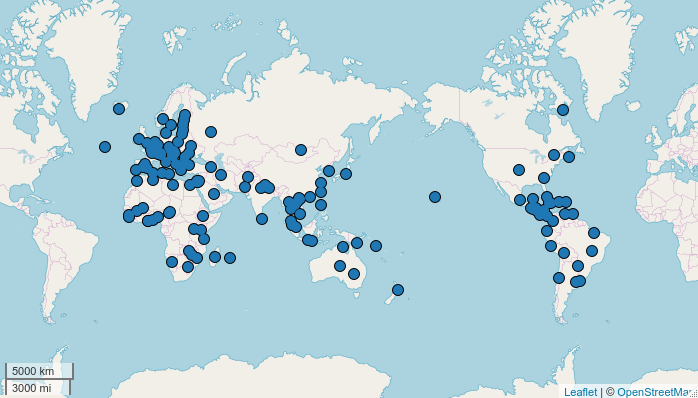
\includegraphics[width=\linewidth]{images/01-sign}
\end{frame}

\begin{frame}{Мифы про ЖЯ:}
\begin{itemize}
    \item ЖЯ --- не один язык, а много языков 
    \item Жестикуляция --- это не ЖЯ \pause
    \item Русский жестовый язык --- это не русский язык, передаваемый жестами \pause
    \item В ЖЯ есть грамматика \pause
    \item Глухонемые? Нет, глухие \pause
    \item Существует жестовый театр, жестовые стихи и жестовое пение
\end{itemize}
\end{frame}

\section{История изучения} % Аня

\begin{frame}{Как все неправильно поняли Аристотеля}
    \begin{description}
        \item[16-ый век] может быть, все были не правы, но это не точно \pause
        \item[конец 18-ого --- начало 19-ого века] Возникновение школ для глухих (а именно 1760-е, Париж, Abbé Charles-Michel de l’Epée)
    \end{description}
\includemovie{2cm}{2cm}{images/delepe.gif}
% AAAAAAAAAAAAAAAAAAAAAAAAAAAAAAAAAAAAAAAAAAAAAAAAAAAAA
% Гарик, оно не работает, помоги, пожалуйста
\end{frame}

\begin{frame}{Как все неправильно поняли Аристотеля}
    \begin{description}
        \item[16-ый век] может быть, все были не правы, но это не точно
        \item[конец 18-ого --- начало 19-ого века] Возникновение школ для глухих (а именно 1760-е, Париж, Abbé Charles-Michel de l’Epée)
        \item[1864] Gallaudet University \pause
        \item[2/2 18-juj]
        \item[1960 год] Стоуки написал первое лингвистическое исследование
    \end{description}
\end{frame}

\section{Грамматические особенности РЖЯ} % Гарик
\begin{frame}{Грамматика РЖЯ}
\begin{itemize}
    \item нет падежей
    \item посессивная конструкция (мой мальчик)
    \item отрицание
\end{itemize}
\end{frame}

\section{Иконичность и одновременность} % Аня
\begin{frame}{Чем жестовые языки принципиально отличаются от звучащих?}
\begin{itemize}
    \item Иконичность
    \item Одновременность
\end{itemize}
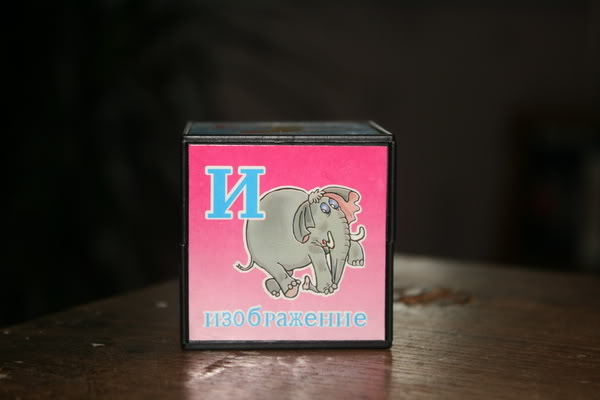
\includegraphics[width=\linewidth]{images/test}
\end{frame}

\section{Фонетика и фонология} % Гарик

\section{Автоматическое распознавание ЖЯ} % Аня
\begin{frame}{Автоматическое распознавание ЖЯ}
    \begin{itemize}
        \item openCV
        \item openPose
    \end{itemize}
\end{frame}

\begin{frame}{OpenPose для распознавания ЖЯ}
    ???
\end{frame}

\begin{frame}{Распознавание русского жестового языка}
    virtually nonexistent
\end{frame}

\section{Песня, стихи и т. п.} % Гарик и Аня
\begin{frame}{Жестовая песня}
    https://www.youtube.com/watch?v=n-lNtm1lKsw
\end{frame}

\begin{frame}{Стихи}
https://www.youtube.com/watch?v=TvN0VwT3BJ8 
Я не уверена что это то, что мы хотим тут рассказывать 
\end{frame}

\end{document}